\documentclass[12pt]{article}
\usepackage{graphicx}
\usepackage[english]{babel}
\usepackage{url}
\usepackage{listings}
\usepackage{color}
\usepackage{subcaption}
\usepackage{tikzscale}
\usepackage{mwe}
\usepackage{xcolor}
\usepackage{tabu}
\usepackage{mathtools}
\usepackage{physics}
\usepackage{amssymb}
\usepackage{pgfplots}
\usepackage{empheq}
\usepackage{float}
\usepackage[font={small,it}]{caption}
\usepackage{tikz}
\usetikzlibrary{decorations.pathreplacing}
\usetikzlibrary{3d}
\usepackage{cancel}
\newcommand{\myparagraph}[1]{\paragraph{#1}\mbox{}\\}
\usepackage{titlesec}
\newcommand{\doubleCross}{%
	\raisebox{-1pt}{%
		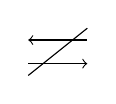
\begin{tikzpicture}[scale = 3]%
		\draw [->] (0, 0) -- (0.25, 0);                 
		\draw [<-] (0, 0.1) -- (0.25, 0.1);     
		\draw [black](0.25,0.15) -- (0,-0.05);  
		\end{tikzpicture}
	}
}

\pgfplotsset{compat=1.16}

\newcommand{\singleCross}{%
	\raisebox{-1pt}{%
		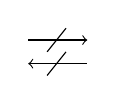
\begin{tikzpicture}[scale = 3]%
		\draw [<-] (0, 0) -- (0.25, 0);            
		\draw [black](0.16,0.15) -- (0.08,0.05);   
		\draw [->] (0, 0.1) -- (0.25, 0.1);       
		\draw [black](0.16,0.05) -- (0.08,-0.05);   
		\end{tikzpicture}
	}
}

% Hyperlinks in contents
\usepackage{hyperref}
\hypersetup{
    colorlinks,
    citecolor=black,
    filecolor=black,
    linkcolor=black,
    urlcolor=black
}
% Make links look great again
\urlstyle{same}

% Silence hyperref warnings about math formulas in sections, make sure to include new characters used
\pdfstringdefDisableCommands{%
%  \def${}%
  \def\alpha{alpha}%
  \def\epsilon{epsilon}%
  \def\gamma{gamma}%
  \def\({}%
  \def\){}%
  \def\texttt#1{<#1>}%
}

\begin{document}

\definecolor{dkgreen}{rgb}{0,0.6,0}
\definecolor{gray}{rgb}{0.5,0.5,0.5}
\definecolor{mauve}{rgb}{0.58,0,0.82}
\definecolor{backcolour}{rgb}{0.95,0.95,0.92}
\definecolor{gray}{rgb}{0.4,0.4,0.4}
\definecolor{darkblue}{rgb}{0.0,0.0,0.6}
\definecolor{cyan}{rgb}{0.0,0.6,0.6}
\definecolor{brightcerulean}{rgb}{0.11, 0.67, 0.84}

\lstset{frame=tb,
  backgroundcolor=\color{backcolour},   
  aboveskip=3mm,
  belowskip=3mm,
  showstringspaces=false,
  columns=flexible,
  basicstyle={\small\ttfamily},
  numbers=none,
  numberstyle=\tiny\color{gray},
  keywordstyle=\color{blue},
  commentstyle=\color{dkgreen},
  stringstyle=\color{mauve},
  breaklines=true,
  breakatwhitespace=true,
  tabsize=3
}
\begin{titlepage}
    \centering
    \includegraphics[width=1\textwidth]{pictures/title.pdf}\par\vspace{0.5cm}
    {\scshape\LARGE Kantonsschule Wohlen \par}
    \vspace{0.2cm}
    {\scshape\Large Matura-project\par}
    \vspace{2cm}
    {\huge\bfseries Creating an AI which can play games\par}
    \vspace{2cm}
    {\Large\itshape Brian Funk und Silvan Metzker\par}
    \vfill
    directed by\par
    Patric \textsc{Rousselot} und Mark \textsc{Heinz}
    \vfill 
    {10. September, 2020}
\end{titlepage}
\tableofcontents
\newpage

\section{Introduction}
The goal of this project is to create an artificial intelligence (AI) which can play games. This is achieved by utilizing a practice called \textit{machine learning}. Machine learning is defined as a technique which can learn by using computational power. It's a generic term mainly used to describe AIs which learn by analysing huge amounts of data. 
The most human-like strategy in machine learning is \textit{deep learning}. It's structure is similar to a human brain and does surprisingly well at mimicking the brain's abilities to learn. In this process we strive to better understand the complexity and functioning of an artificial human-like brain. 
\section{Basics of Artificial Intelligence}
\subsection{What is an AI}
An Artificial Intelligence, in short AI, is the ability of a digital device to execute tasks which are related to human beings and animals. This vague description can be taken in many ways so a closer description would be a \textit{Narrow AI}. \cite{aibritannica}\\
Artificial Narrow AI (ANI) is a type of AI which can only be applied to one narrow task. This is the kind of AI that currently exists. It can do a task very well, even better than humans. For example an AI that detects brain tumors way more accurately than a experienced neurosurgeon is expected to. It's revolutionary and does very well at one certain task, regardless it cannot tell the difference between a cat and a dog. This is considered as an Artifcial Narrow Intelligence. An Artificial General Intelligence (AGI) on the other hand is an AI that can perform all tasks a human can fulfil. This type of AI is not yet discovered. The step after that would be a Artificial Super Intelligence (ASI), this is the kind of AI that is superior in every way a human. It is also considered as the type of AI that could possibly lead to the extinction of the human race. The closest approach to one of those higher levels of a AI was achieved by one of the so called artificial neuronal networks (ANNs).
\cite{narrowAI}
\subsection{Mathematics behind a neuronal network}
\subsubsection{Neuronal network}\label{sec:nnmath}
A model which is used for many self-learning applications is called \textit{neuronal network}. 
This model mimics the human brain and tries to describe the learning-behaviour as accurate as possible. Although it has biological foundations it can be described in a purely mathematical way. To understand this certain terms have to be defined mathematically and linguistically.
As in the brain a \textit{neuron} takes multiple inputs and passes forward an output, which is somehow dependant on the input. The human brain uses electric current to transfer information. The AI does this numerically. The inputs are multiplied by a certain factor. Later in the learning process these factors are the values that are going to be optimized and changed. By increasing or decreasing these values one node can have more or less impact. The neuron takes all the inputs and adds them together. This sum gets forwarded to the \textit{activation function}, which calculates the respective value. This transformed value gets weighted and gets passed to the output or to a new neuron in the next \textit{layer}. Two neurons can make a connection, which is used to pass the numerical outputs of the function into the next neuron. These neurons build up \textit{layers} and determine its size with the amount of neurons. One of the properties of the layer is, that all neurons from one layer don't connect to each other. But they do connect to the previous and subsequent layer. The layer can be categorized in three different kinds: input, output and hidden layers. The hidden layer describes all layers, except the in- and output layers. \cite{neuronal_network}\\
\begin{figure}[H]
\begin{center}

\tikzset{every picture/.style={line width=0.75pt}} %set default line width to 0.75pt        

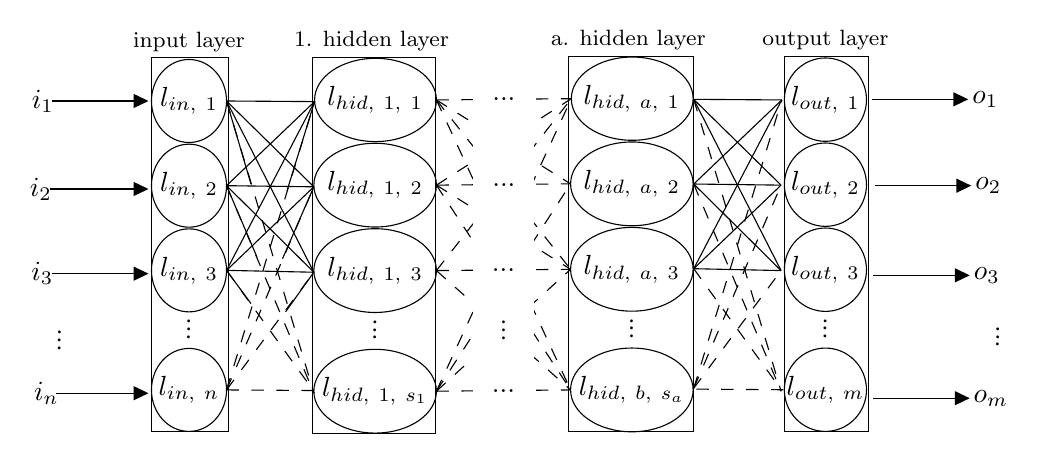
\begin{tikzpicture}[x=0.75pt,y=0.75pt,yscale=-0.8,xscale=0.8]
%uncomment if require: \path (0,300); %set diagram left start at 0, and has height of 300

%Shape: Rectangle [id:dp5348683704419017] 
\draw   (76.28,62) -- (122.66,62) -- (122.66,287) -- (76.28,287) -- cycle ;
%Shape: Ellipse [id:dp939731478529126] 
\draw   (76.28,88) .. controls (76.28,74.19) and (86.4,63) .. (98.88,63) .. controls (111.36,63) and (121.49,74.19) .. (121.49,88) .. controls (121.49,101.81) and (111.36,113) .. (98.88,113) .. controls (86.4,113) and (76.28,101.81) .. (76.28,88) -- cycle ;
%Shape: Ellipse [id:dp5664589230881223] 
\draw   (76.28,139) .. controls (76.28,125.19) and (86.4,114) .. (98.88,114) .. controls (111.36,114) and (121.49,125.19) .. (121.49,139) .. controls (121.49,152.81) and (111.36,164) .. (98.88,164) .. controls (86.4,164) and (76.28,152.81) .. (76.28,139) -- cycle ;

%Shape: Ellipse [id:dp7228345414575519] 
\draw   (76.28,190) .. controls (76.28,176.19) and (86.4,165) .. (98.88,165) .. controls (111.36,165) and (121.49,176.19) .. (121.49,190) .. controls (121.49,203.81) and (111.36,215) .. (98.88,215) .. controls (86.4,215) and (76.28,203.81) .. (76.28,190) -- cycle ;

%Shape: Ellipse [id:dp6381471751303389] 
\draw   (76.28,262) .. controls (76.28,248.19) and (86.4,237) .. (98.88,237) .. controls (111.36,237) and (121.49,248.19) .. (121.49,262) .. controls (121.49,275.81) and (111.36,287) .. (98.88,287) .. controls (86.4,287) and (76.28,275.81) .. (76.28,262) -- cycle ;

%Straight Lines [id:da0033305459292130024] 
\draw    (16.49,88) -- (71.47,88) ;
\draw [shift={(74.47,88)}, rotate = 180] [fill={rgb, 255:red, 0; green, 0; blue, 0 }  ][line width=0.08]  [draw opacity=0] (8.93,-4.29) -- (0,0) -- (8.93,4.29) -- cycle    ;

%Straight Lines [id:da5101048873615364] 
\draw    (15.34,141) -- (71.47,141) ;
\draw [shift={(74.47,141)}, rotate = 180] [fill={rgb, 255:red, 0; green, 0; blue, 0 }  ][line width=0.08]  [draw opacity=0] (8.93,-4.29) -- (0,0) -- (8.93,4.29) -- cycle    ;

%Straight Lines [id:da6465200926879782] 
\draw    (16.21,192) -- (71.47,192) ;
\draw [shift={(74.47,192)}, rotate = 180] [fill={rgb, 255:red, 0; green, 0; blue, 0 }  ][line width=0.08]  [draw opacity=0] (8.93,-4.29) -- (0,0) -- (8.93,4.29) -- cycle    ;

%Straight Lines [id:da5162655773532001] 
\draw    (19.05,264) -- (71.47,264) ;
\draw [shift={(74.47,264)}, rotate = 180] [fill={rgb, 255:red, 0; green, 0; blue, 0 }  ][line width=0.08]  [draw opacity=0] (8.93,-4.29) -- (0,0) -- (8.93,4.29) -- cycle    ;

%Shape: Rectangle [id:dp18972253282167162] 
\draw   (173.05,62) -- (247.44,62) -- (247.44,288) -- (173.05,288) -- cycle ;
%Shape: Ellipse [id:dp7229152371524696] 
\draw   (174.52,87.37) .. controls (174.52,73.53) and (190.94,62.3) .. (211.2,62.3) .. controls (231.46,62.3) and (247.88,73.53) .. (247.88,87.37) .. controls (247.88,101.22) and (231.46,112.45) .. (211.2,112.45) .. controls (190.94,112.45) and (174.52,101.22) .. (174.52,87.37) -- cycle ;
%Shape: Ellipse [id:dp5195092025670933] 
\draw   (174.08,138.68) .. controls (174.08,124.75) and (190.6,113.46) .. (210.98,113.46) .. controls (231.36,113.46) and (247.88,124.75) .. (247.88,138.68) .. controls (247.88,152.61) and (231.36,163.9) .. (210.98,163.9) .. controls (190.6,163.9) and (174.08,152.61) .. (174.08,138.68) -- cycle ;
%Shape: Ellipse [id:dp45163062887236016] 
\draw   (174.08,190.13) .. controls (174.08,176.2) and (190.6,164.91) .. (210.98,164.91) .. controls (231.36,164.91) and (247.88,176.2) .. (247.88,190.13) .. controls (247.88,204.06) and (231.36,215.36) .. (210.98,215.36) .. controls (190.6,215.36) and (174.08,204.06) .. (174.08,190.13) -- cycle ;
%Shape: Ellipse [id:dp6104698680122025] 
\draw   (174.08,262.78) .. controls (174.08,248.85) and (190.6,237.55) .. (210.98,237.55) .. controls (231.36,237.55) and (247.88,248.85) .. (247.88,262.78) .. controls (247.88,276.71) and (231.36,288) .. (210.98,288) .. controls (190.6,288) and (174.08,276.71) .. (174.08,262.78) -- cycle ;
%Shape: Rectangle [id:dp3256666346119699] 
\draw   (327.67,61.22) -- (402.96,61.22) -- (402.96,287.22) -- (327.67,287.22) -- cycle ;
%Shape: Ellipse [id:dp5309517723311545] 
\draw   (329.14,86.6) .. controls (329.14,72.75) and (345.56,61.53) .. (365.82,61.53) .. controls (386.07,61.53) and (402.49,72.75) .. (402.49,86.6) .. controls (402.49,100.44) and (386.07,111.67) .. (365.82,111.67) .. controls (345.56,111.67) and (329.14,100.44) .. (329.14,86.6) -- cycle ;
%Shape: Ellipse [id:dp4644453089406313] 
\draw   (328.7,137.9) .. controls (328.7,123.97) and (345.22,112.68) .. (365.6,112.68) .. controls (385.97,112.68) and (402.49,123.97) .. (402.49,137.9) .. controls (402.49,151.83) and (385.97,163.13) .. (365.6,163.13) .. controls (345.22,163.13) and (328.7,151.83) .. (328.7,137.9) -- cycle ;
%Shape: Ellipse [id:dp8559292750865175] 
\draw   (328.7,189.36) .. controls (328.7,175.43) and (345.22,164.13) .. (365.6,164.13) .. controls (385.97,164.13) and (402.49,175.43) .. (402.49,189.36) .. controls (402.49,203.29) and (385.97,214.58) .. (365.6,214.58) .. controls (345.22,214.58) and (328.7,203.29) .. (328.7,189.36) -- cycle ;
%Shape: Ellipse [id:dp1970629242881392] 
\draw   (328.7,262) .. controls (328.7,248.07) and (345.22,236.78) .. (365.6,236.78) .. controls (385.97,236.78) and (402.49,248.07) .. (402.49,262) .. controls (402.49,275.93) and (385.97,287.22) .. (365.6,287.22) .. controls (345.22,287.22) and (328.7,275.93) .. (328.7,262) -- cycle ;
%Shape: Rectangle [id:dp7142888753284027] 
\draw   (457.44,61.09) -- (508.19,61.09) -- (508.19,287) -- (457.44,287) -- cycle ;
%Shape: Ellipse [id:dp7295760206982997] 
\draw   (457.44,87.19) .. controls (457.44,73.33) and (468.51,62.09) .. (482.17,62.09) .. controls (495.83,62.09) and (506.9,73.33) .. (506.9,87.19) .. controls (506.9,101.05) and (495.83,112.29) .. (482.17,112.29) .. controls (468.51,112.29) and (457.44,101.05) .. (457.44,87.19) -- cycle ;
%Shape: Ellipse [id:dp4100384195259268] 
\draw   (457.44,138.4) .. controls (457.44,124.54) and (468.51,113.3) .. (482.17,113.3) .. controls (495.83,113.3) and (506.9,124.54) .. (506.9,138.4) .. controls (506.9,152.26) and (495.83,163.5) .. (482.17,163.5) .. controls (468.51,163.5) and (457.44,152.26) .. (457.44,138.4) -- cycle ;

%Shape: Ellipse [id:dp7445535886007981] 
\draw   (457.44,189.61) .. controls (457.44,175.74) and (468.51,164.5) .. (482.17,164.5) .. controls (495.83,164.5) and (506.9,175.74) .. (506.9,189.61) .. controls (506.9,203.47) and (495.83,214.71) .. (482.17,214.71) .. controls (468.51,214.71) and (457.44,203.47) .. (457.44,189.61) -- cycle ;

%Shape: Ellipse [id:dp5696755418086674] 
\draw   (457.44,261.9) .. controls (457.44,248.04) and (468.51,236.8) .. (482.17,236.8) .. controls (495.83,236.8) and (506.9,248.04) .. (506.9,261.9) .. controls (506.9,275.76) and (495.83,287) .. (482.17,287) .. controls (468.51,287) and (457.44,275.76) .. (457.44,261.9) -- cycle ;
%Straight Lines [id:da18885212790099604] 
\draw    (511.09,267) -- (566.07,267) ;
\draw [shift={(569.07,267)}, rotate = 180] [fill={rgb, 255:red, 0; green, 0; blue, 0 }  ][line width=0.08]  [draw opacity=0] (8.93,-4.29) -- (0,0) -- (8.93,4.29) -- cycle    ;

%Straight Lines [id:da35087841460038605] 
\draw    (510.19,87) -- (565.16,87) ;
\draw [shift={(568.16,87)}, rotate = 180] [fill={rgb, 255:red, 0; green, 0; blue, 0 }  ][line width=0.08]  [draw opacity=0] (8.93,-4.29) -- (0,0) -- (8.93,4.29) -- cycle    ;

%Straight Lines [id:da5340215529143741] 
\draw    (511.99,139) -- (566.97,139) ;
\draw [shift={(569.97,139)}, rotate = 180] [fill={rgb, 255:red, 0; green, 0; blue, 0 }  ][line width=0.08]  [draw opacity=0] (8.93,-4.29) -- (0,0) -- (8.93,4.29) -- cycle    ;

%Straight Lines [id:da6816101523134108] 
\draw    (511.09,193) -- (566.07,193) ;
\draw [shift={(569.07,193)}, rotate = 180] [fill={rgb, 255:red, 0; green, 0; blue, 0 }  ][line width=0.08]  [draw opacity=0] (8.93,-4.29) -- (0,0) -- (8.93,4.29) -- cycle    ;

%Straight Lines [id:da07173699686933155] 
\draw  [dash pattern={on 4.5pt off 4.5pt}]  (121.49,88) -- (174.08,263.78) ;
%Straight Lines [id:da6699097779078262] 
\draw  [dash pattern={on 4.5pt off 4.5pt}]  (121.49,262) -- (174.08,191.13) ;
%Straight Lines [id:da1642802446958136] 
\draw  [dash pattern={on 4.5pt off 4.5pt}]  (121.49,262) -- (174.08,139.68) ;
%Straight Lines [id:da1882795920867577] 
\draw  [dash pattern={on 4.5pt off 4.5pt}]  (121.49,262) -- (174.52,88.37) ;
%Straight Lines [id:da21393539615592538] 
\draw    (121.49,88) -- (174.52,88.37) ;
%Straight Lines [id:da4487867895893247] 
\draw    (121.49,88) -- (174.08,139.68) ;
%Straight Lines [id:da07147649974582793] 
\draw    (121.49,88) -- (174.08,191.13) ;
%Straight Lines [id:da29330792079044166] 
\draw    (121.49,139) -- (174.52,88.37) ;
%Straight Lines [id:da49448158210002213] 
\draw  [dash pattern={on 4.5pt off 4.5pt}]  (121.49,190) -- (174.08,262.78) ;
%Straight Lines [id:da09798373867862575] 
\draw    (121.49,139) -- (174.08,191.13) ;
%Straight Lines [id:da5600404631656062] 
\draw  [dash pattern={on 4.5pt off 4.5pt}]  (121.49,139) -- (174.08,263.78) ;
%Straight Lines [id:da7057392759609711] 
\draw    (121.49,190) -- (174.52,88.37) ;
%Straight Lines [id:da2885366017727522] 
\draw    (121.49,190) -- (174.08,139.68) ;
%Straight Lines [id:da34302481014830266] 
\draw    (121.49,190) -- (174.08,191.13) ;
%Straight Lines [id:da3967598060261417] 
\draw    (121.49,139) -- (174.08,139.68) ;
%Straight Lines [id:da2561105605921401] 
\draw    (121.49,88) -- (136.22,138) ;
%Straight Lines [id:da0846780391827735] 
\draw    (174.52,88.37) -- (157.92,142) ;
%Straight Lines [id:da8561394015640085] 
\draw    (174.08,139.68) -- (155.21,183) ;
%Straight Lines [id:da7742955999004255] 
\draw    (174.08,191.13) -- (157.02,215) ;
%Straight Lines [id:da3741138292647084] 
\draw    (121.49,139) -- (139.84,182) ;
%Straight Lines [id:da19823177683211468] 
\draw    (121.49,190) -- (136.22,210) ;
%Straight Lines [id:da7799354395016436] 
\draw  [dash pattern={on 4.5pt off 4.5pt}]  (247.88,87.37) -- (329.14,86.6) ;
%Straight Lines [id:da8112635885919046] 
\draw  [dash pattern={on 4.5pt off 4.5pt}]  (247.88,87.37) -- (328.7,137.9) ;
%Straight Lines [id:da43416826759224025] 
\draw  [dash pattern={on 4.5pt off 4.5pt}]  (247.88,87.37) -- (328.7,189.36) ;
%Straight Lines [id:da5962912105851825] 
\draw  [dash pattern={on 4.5pt off 4.5pt}]  (247.88,87.37) -- (328.7,262) ;
%Straight Lines [id:da414758159631222] 
\draw  [dash pattern={on 4.5pt off 4.5pt}]  (247.88,138.68) -- (328.7,137.9) ;
%Straight Lines [id:da4655355837425297] 
\draw  [dash pattern={on 4.5pt off 4.5pt}]  (247.88,138.68) -- (329.14,86.6) ;
%Straight Lines [id:da19554879472652642] 
\draw  [dash pattern={on 4.5pt off 4.5pt}]  (247.88,138.68) -- (328.7,189.36) ;
%Straight Lines [id:da5323232176676549] 
\draw  [dash pattern={on 4.5pt off 4.5pt}]  (247.88,138.68) -- (328.7,262) ;
%Straight Lines [id:da6152630037551357] 
\draw  [dash pattern={on 4.5pt off 4.5pt}]  (247.88,190.13) -- (329.14,86.6) ;
%Straight Lines [id:da7928666915958094] 
\draw  [dash pattern={on 4.5pt off 4.5pt}]  (247.88,190.13) -- (328.7,262) ;
%Straight Lines [id:da37586727330985115] 
\draw  [dash pattern={on 4.5pt off 4.5pt}]  (247.88,190.13) -- (328.7,189.36) ;
%Straight Lines [id:da7715167325292387] 
\draw  [dash pattern={on 4.5pt off 4.5pt}]  (247.88,262.78) -- (328.7,262) ;
%Straight Lines [id:da8147553751065622] 
\draw  [dash pattern={on 4.5pt off 4.5pt}]  (247.88,262.78) -- (328.7,189.36) ;
%Straight Lines [id:da8607258541912663] 
\draw  [dash pattern={on 4.5pt off 4.5pt}]  (247.88,262.78) -- (328.7,137.9) ;
%Straight Lines [id:da4710290973854665] 
\draw  [dash pattern={on 4.5pt off 4.5pt}]  (247.88,262.78) -- (329.14,86.6) ;
%Shape: Rectangle [id:dp8707492920309927] 
\draw  [draw opacity=0][fill={rgb, 255:red, 255; green, 255; blue, 255 }  ,fill opacity=1 ] (269.75,74.69) -- (306.82,74.69) -- (306.82,274.69) -- (269.75,274.69) -- cycle ;
%Straight Lines [id:da789374598203767] 
\draw  [dash pattern={on 4.5pt off 4.5pt}]  (402.86,87) -- (455.46,262.78) ;
%Straight Lines [id:da5608607968941501] 
\draw  [dash pattern={on 4.5pt off 4.5pt}]  (402.86,261) -- (455.46,190.13) ;
%Straight Lines [id:da8173621393477881] 
\draw  [dash pattern={on 4.5pt off 4.5pt}]  (402.86,261) -- (455.46,138.68) ;
%Straight Lines [id:da42024579143459984] 
\draw  [dash pattern={on 4.5pt off 4.5pt}]  (402.86,261) -- (455.9,87.37) ;
%Straight Lines [id:da4970992533092691] 
\draw    (402.86,87) -- (455.9,87.37) ;
%Straight Lines [id:da5336499941942965] 
\draw    (402.86,87) -- (455.46,138.68) ;
%Straight Lines [id:da6837746318616225] 
\draw    (402.86,87) -- (455.46,190.13) ;
%Straight Lines [id:da2450666544795037] 
\draw    (402.86,138) -- (455.9,87.37) ;
%Straight Lines [id:da54432464900309] 
\draw  [dash pattern={on 4.5pt off 4.5pt}]  (402.86,189) -- (455.46,261.78) ;
%Straight Lines [id:da9110502437081351] 
\draw    (402.86,138) -- (455.46,190.13) ;
%Straight Lines [id:da18057385661891412] 
\draw  [dash pattern={on 4.5pt off 4.5pt}]  (402.86,138) -- (455.46,262.78) ;
%Straight Lines [id:da613380831677923] 
\draw    (402.86,189) -- (455.9,87.37) ;
%Straight Lines [id:da6296455944188728] 
\draw    (402.86,189) -- (455.46,138.68) ;
%Straight Lines [id:da11572374477508784] 
\draw    (402.86,189) -- (455.46,190.13) ;
%Straight Lines [id:da17311782425039035] 
\draw    (402.86,138) -- (455.46,138.68) ;

%Straight Lines [id:da6430113077352528] 
\draw  [dash pattern={on 4.5pt off 4.5pt}]  (121.49,262) -- (174.52,262.37) ;
%Straight Lines [id:da7394517258615123] 
\draw  [dash pattern={on 4.5pt off 4.5pt}]  (404.4,261.52) -- (457.44,261.9) ;

% Text Node
\draw (570.06,193) node [anchor=west] [inner sep=0.75pt]   [align=left] {$\displaystyle o_{3}$};
% Text Node
\draw (570.96,139) node [anchor=west] [inner sep=0.75pt]   [align=left] {$\displaystyle o_{2}$};
% Text Node
\draw (569.16,87) node [anchor=west] [inner sep=0.75pt]   [align=left] {$\displaystyle o_{1}$};
% Text Node
\draw (569.87,267) node [anchor=west] [inner sep=0.75pt]   [align=left] {$\displaystyle o_{m}$};
% Text Node
\draw (482.17,189.61) node   [align=left] {$\displaystyle l_{out,\ 3}$};
% Text Node
\draw (482.17,138.4) node   [align=left] {$\displaystyle l_{out,\ 2}$};
% Text Node
\draw (22.03,264) node [anchor=east] [inner sep=0.75pt]   [align=left] {$\displaystyle i_{n}$};
% Text Node
\draw (18.72,192) node [anchor=east] [inner sep=0.75pt]   [align=left] {$\displaystyle i_{3}$};
% Text Node
\draw (17.78,141) node [anchor=east] [inner sep=0.75pt]   [align=left] {$\displaystyle i_{2}$};
% Text Node
\draw (19.02,88) node [anchor=east] [inner sep=0.75pt]   [align=left] {$\displaystyle i_{1}$};
% Text Node
\draw (98.88,262) node   [align=left] {$\displaystyle l_{in,\ n}$};
% Text Node
\draw (98.88,190) node   [align=left] {$\displaystyle l_{in,\ 3}$};
% Text Node
\draw (98.88,139) node   [align=left] {$\displaystyle l_{in,\ 2}$};
% Text Node
\draw (98.88,88) node   [align=left] {$\displaystyle l_{in,\ 1}$};
% Text Node
\draw (482.14,216.71) node [anchor=west] [inner sep=0.75pt]  [rotate=-91.1] [align=left] {...};
% Text Node
\draw (482.17,59.04) node [anchor=south] [inner sep=0.75pt]  [font=\footnotesize] [align=left] {output layer};
% Text Node
\draw (482.17,261.9) node   [align=left] {$\displaystyle l_{out,\ m}$};
% Text Node
\draw (482.17,87.19) node   [align=left] {$\displaystyle l_{out,\ 1}$};
% Text Node
\draw (365.6,86.45) node   [align=left] {$\displaystyle l_{hid,\ a,\ 1}$};
% Text Node
\draw (365.6,137.9) node   [align=left] {$\displaystyle l_{hid,\ a,\ 2}$};
% Text Node
\draw (365.6,189.36) node   [align=left] {$\displaystyle l_{hid,\ a,\ 3}$};
% Text Node
\draw (365.6,262) node   [align=left] {$\displaystyle l_{hid,\ b,\ s_{a}}$};
% Text Node
\draw (365.43,216.58) node [anchor=west] [inner sep=0.75pt]  [rotate=-90] [align=left] {...};
% Text Node
\draw (365.82,58.53) node [anchor=south] [inner sep=0.75pt]  [font=\footnotesize] [align=left] {a. hidden layer };
% Text Node
\draw (210.95,217.36) node [anchor=west] [inner sep=0.75pt]  [rotate=-91.1] [align=left] {...};
% Text Node
\draw (210.98,262.78) node   [align=left] {$\displaystyle l_{hid,\ 1,\ s_{1}}$};
% Text Node
\draw (210.98,190.13) node   [align=left] {$\displaystyle l_{hid,\ 1,\ 3}$};
% Text Node
\draw (210.98,138.68) node   [align=left] {$\displaystyle l_{hid,\ 1,\ 2}$};
% Text Node
\draw (210.98,87.22) node   [align=left] {$\displaystyle l_{hid,\ 1,\ 1}$};
% Text Node
\draw (211.2,59.3) node [anchor=south] [inner sep=0.75pt]  [font=\footnotesize] [align=left] {1. hidden layer };
% Text Node
\draw (588.55,221.66) node [anchor=north west][inner sep=0.75pt]  [rotate=-91.1] [align=left] {...};
% Text Node
\draw (23.42,223.66) node [anchor=north west][inner sep=0.75pt]  [rotate=-91.1] [align=left] {...};
% Text Node
\draw (98.85,217) node [anchor=west] [inner sep=0.75pt]  [rotate=-91.1] [align=left] {...};
% Text Node
\draw (98.88,60) node [anchor=south] [inner sep=0.75pt]  [font=\footnotesize] [align=left] {input layer};
% Text Node
\draw (288.51,86.99) node   [align=left] {...};
% Text Node
\draw (288.51,138.37) node   [align=left] {...};
% Text Node
\draw (288.29,189.75) node   [align=left] {...};
% Text Node
\draw (288.29,262.39) node   [align=left] {...};
% Text Node
\draw (288.29,226.07) node  [rotate=-90.15] [align=left] {...};


\end{tikzpicture}


\end{center}
\caption{The relation between the different layers.}
\label{neuronal_layer_relation}
\end{figure}

The neuronal network consists of all parts mentioned before, as it can be seen in figure \ref{neuronal_layer_relation}. The first layer is the input layer and has as many nodes, as the input size $n$. Which means if you want to forward binary information of four variables, the input size and therefore the input layer would be the size of four neurons. This also holds for the output layer size, which is denoted by $m$. 
The amount of hidden layers $a$ and its size $s$ can be chosen arbitrarily. Although there are no constraints for the hidden layers, the amount and size can hugely affect the efficiency and capability to learn. Every circle or ellipse represents one neuron. 
\begin{figure}[H]
\begin{center}
\label{neuron}
\tikzset{every picture/.style={line width=0.75pt}} %set default line width to 0.75pt    
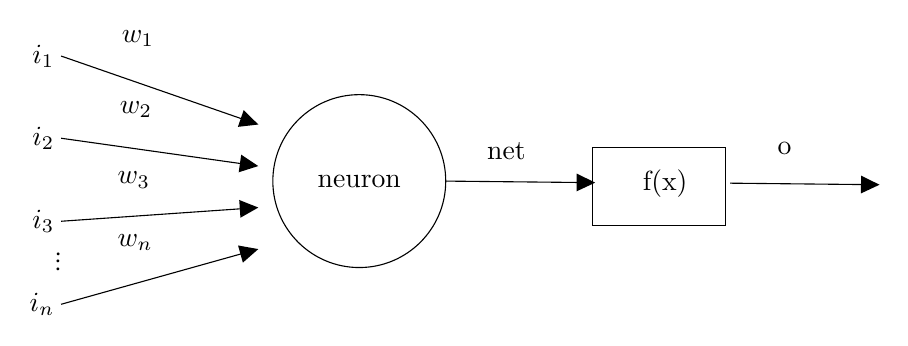
\begin{tikzpicture}[x=0.75pt,y=0.75pt,yscale=-1,xscale=1]
%uncomment if require: \path (0,300); %set diagram left start at 0, and has height of 300

%Shape: Circle [id:dp8788298950890718] 
\draw   (226,121.65) .. controls (226,98.65) and (244.65,80) .. (267.65,80) .. controls (290.65,80) and (309.3,98.65) .. (309.3,121.65) .. controls (309.3,144.65) and (290.65,163.3) .. (267.65,163.3) .. controls (244.65,163.3) and (226,144.65) .. (226,121.65) -- cycle ;
%Straight Lines [id:da3838769529758834] 
\draw    (124,101) -- (216.03,113.98) ;
\draw [shift={(219,114.4)}, rotate = 188.03] [fill={rgb, 255:red, 0; green, 0; blue, 0 }  ][line width=0.08]  [draw opacity=0] (8.93,-4.29) -- (0,0) -- (8.93,4.29) -- cycle    ;
%Straight Lines [id:da23619311043896896] 
\draw    (124,141) -- (216.01,134.61) ;
\draw [shift={(219,134.4)}, rotate = 536.03] [fill={rgb, 255:red, 0; green, 0; blue, 0 }  ][line width=0.08]  [draw opacity=0] (8.93,-4.29) -- (0,0) -- (8.93,4.29) -- cycle    ;
%Straight Lines [id:da4533097231798262] 
\draw    (124,181) -- (216.11,155.21) ;
\draw [shift={(219,154.4)}, rotate = 524.36] [fill={rgb, 255:red, 0; green, 0; blue, 0 }  ][line width=0.08]  [draw opacity=0] (8.93,-4.29) -- (0,0) -- (8.93,4.29) -- cycle    ;
%Straight Lines [id:da017364411003136793] 
\draw    (124,61.4) -- (216.17,93.42) ;
\draw [shift={(219,94.4)}, rotate = 199.16] [fill={rgb, 255:red, 0; green, 0; blue, 0 }  ][line width=0.08]  [draw opacity=0] (8.93,-4.29) -- (0,0) -- (8.93,4.29) -- cycle    ;
%Straight Lines [id:da2738426817104591] 
\draw    (309.3,121.65) -- (378.3,122.37) ;
\draw [shift={(381.3,122.4)}, rotate = 180.6] [fill={rgb, 255:red, 0; green, 0; blue, 0 }  ][line width=0.08]  [draw opacity=0] (8.93,-4.29) -- (0,0) -- (8.93,4.29) -- cycle    ;
%Shape: Rectangle [id:dp15584865208252952] 
\draw   (380,105.4) -- (444.3,105.4) -- (444.3,143) -- (380,143) -- cycle ;
%Straight Lines [id:da6312953564844079] 
\draw    (446.3,122.65) -- (515.3,123.37) ;
\draw [shift={(518.3,123.4)}, rotate = 180.6] [fill={rgb, 255:red, 0; green, 0; blue, 0 }  ][line width=0.08]  [draw opacity=0] (8.93,-4.29) -- (0,0) -- (8.93,4.29) -- cycle    ;

% Text Node
\draw (267.65,121.65) node   [align=left] {neuron};
% Text Node
\draw (122,61.4) node [anchor=east] [inner sep=0.75pt]   [align=left] {$\displaystyle i_{1}$};
% Text Node
\draw (122,141) node [anchor=east] [inner sep=0.75pt]   [align=left] {$\displaystyle i_{3}$};
% Text Node
\draw (122,101) node [anchor=east] [inner sep=0.75pt]   [align=left] {$\displaystyle i_{2}$};
% Text Node
\draw (122,181) node [anchor=east] [inner sep=0.75pt]   [align=left] {$\displaystyle i_{n}$};
% Text Node
\draw (124.63,153.66) node [anchor=north west][inner sep=0.75pt]  [rotate=-91.1] [align=left] {...};
% Text Node
\draw (152,48) node [anchor=north west][inner sep=0.75pt]   [align=left] {$\displaystyle w_{1}$};
% Text Node
\draw (151,82) node [anchor=north west][inner sep=0.75pt]   [align=left] {$\displaystyle w_{2}$};
% Text Node
\draw (150,146) node [anchor=north west][inner sep=0.75pt]   [align=left] {$\displaystyle w_{n}$};
% Text Node
\draw (150,116) node [anchor=north west][inner sep=0.75pt]   [align=left] {$\displaystyle w_{3}$};
% Text Node
\draw (415,123) node   [align=left] {f(x)};
% Text Node
\draw (468,102) node [anchor=north west][inner sep=0.75pt]   [align=left] {o};
% Text Node
\draw (328,102) node [anchor=north west][inner sep=0.75pt]   [align=left] {net};
\end{tikzpicture}
\caption{A visualization of a neuron.}
\label{neuron_vis}
\end{center}
\end{figure}
In figure \ref{neuron_vis} the structure of a neuron can be seen. The abbreviation $i$ stands for input, $w$ refers to weight and $o$ to the output of the neuron. The inputs and weights can be described in the form of a \textit{vector}. The output $o$ gets weighted accordingly and functions as input for the following neurons. Each component represents one input or weight. This yields the vectors $\vec{i}$ and $\vec{w}$.
\begin{align}
\vec{i} = \begin{pmatrix}
i_{1}\\ 
i_{2}\\ 
\ldots \\ 
i_{n}
\end{pmatrix}
&&
\vec{w} = \begin{pmatrix}
w_{1}\\ 
w_{2}\\ 
\ldots \\ 
w_{n}
\end{pmatrix}
\label{def_vector}
\end{align}
The sum, in equation \ref{neuron_vis} referenced as net, is determined by the weighted summation of all the inputs. 
\begin{equation}
  \sum_{x = 1}^{n} i_{x} \cdot w_{x}  
  \label{net_sum}
\end{equation}
The equation \ref{net_sum} shows the net value in the form of a sum.
Due to the properties of the \textit{scalar product} this sum can be rewritten in the form of this vector operation
\begin{equation}
net = \vec{i} \cdot \vec{w}
\label{net_scal}
\end{equation}
This weighted sum gets forwarded to the activation function. By replacing the net value with the definition stated in equation \ref{net_scal}  and $f(x)$ being the activation function, the output is defined as follows:
\begin{equation}
\begin{gathered}
       o = f(net)\\
    o = f(\vec{i} \cdot \vec{w}) 
\end{gathered}
\end{equation}
The final output or an intermediate result of a hidden layer can be expressed in a vector form.
\begin{equation}
\begin{gathered}
      \begin{pmatrix}
o_{1}\\ 
o_{2}\\ 
...\\ 
o_{m}
\end{pmatrix} = \begin{pmatrix}
f(net_{1})\\ 
f(net_{2})\\ 
...\\ 
f(net_{m})
\end{pmatrix}
\end{gathered}
\end{equation}
As we have seen in formula \ref{net_scal} the net value can also be described in a vector form. By expanding the stated definition it can be formulated, such that multiple values are defined in one vector. Although it yields the same result, the output vector $\vec{o}$ can be calculated easier when using net values in a vector form.
\begin{equation}
    \begin{pmatrix}net_{1}\\ net_{2}\\ ...\\ net_{m}\end{pmatrix} =\begin{pmatrix}
w_{1, 1} & w_{2, 1}  & ... &w_{n,1} \\ 
w_{1, 2} & w_{2, 2} & ... & w_{n,2} \\ 
... & ... &  ... & ...\\ 
w_{1,s} & w_{2, s} & ...  & w_{n, s}
\end{pmatrix} \cdot \begin{pmatrix}
i_{1}\\ 
i_{2}\\ 
...\\
i_{n}
\end{pmatrix}
\label{out_vector}
\end{equation}
The formula \ref{out_vector} is a stacked up version of equation \ref{net_scal}. Every row represents all the weights from one specific neuron.The output of this neuron is used as input in the next one. It acts as output as well as an input, but nevertheless it is denoted by $i$. A noticeable remark is, that it fits with the definition of the scalar product, which requires the dimension of the first vector to be the same as the dimension of the second vector. Which is the case as it can be seen. The letter $s$ denotes the size of the layer which the output gets calculated of.
However there are different kinds of neurons depending on their activation functions. Depending on the context, different functions are more efficient to use. The most common and popular types of such are:  \cite{neuronal_network}
\begin{figure}[H]\label{activation_function}
\begin{minipage}[t]{0.5\textwidth}
\begin{center}
\textbf{Linear}
\begin{equation}
    f(x) = x
\end{equation}\newline
\begin{tikzpicture}[scale = 0.5]
\begin{axis}[
  axis x line=center,
  axis y line=center,
  xlabel={$x$},
  ylabel={$y$},
  xlabel style={below right},
  ylabel style={above left},
  xmin=-3,
  xmax=3,
  ymin=-3,
  ymax=3]
\addplot [mark=none,domain=-2.5:2.5] {x};
\end{axis}
\end{tikzpicture}\\
Mostly used in input layers.
\end{center}
\end{minipage}
\begin{minipage}[t]{0.5\textwidth}
\begin{center}
\textbf{Sigmoid}
\begin{equation}
    f(x) = \frac{1}{1 + e^{-x}}
\end{equation}
\begin{tikzpicture}[scale = 0.5]
\begin{axis}[
  axis x line=center,
  axis y line=center,
  xlabel={$x$},
  ylabel={$y$},
  xlabel style={below right},
  ylabel style={above left},
  xmin=-3.5,
  xmax=3.5,
  ymin=-3.5,
  ymax=3.5]
\addplot [mark=none,domain=-3:3] {1/(1+(e^-x))};
\end{axis}
\end{tikzpicture}\\
Mostly used in hidden layers.
\end{center}
\end{minipage}

\vspace{1cm}
\begin{minipage}[t]{0.5\textwidth}
\begin{center}
\textbf{Rectified linear unit (ReLU)}
\begin{equation}
f(x) \left\{\begin{matrix}
0 \text{ for } x \leq 0\\ 
x \text{ for } x >  0
\end{matrix}\right.
\end{equation}
\begin{tikzpicture}[scale = 0.5]
\begin{axis}[
  axis x line=center,
  axis y line=center,
  xlabel={$x$},
  ylabel={$y$},
  xlabel style={below right},
  ylabel style={above left},
  xmin=-3,
  xmax=3,
  ymin=-3,
  ymax=3]
\addplot [mark=none,domain=-2.5:0] {0};
\addplot [mark=none,domain=0:2.5] {x};
\end{axis}
\end{tikzpicture}\\
Mostly used in hidden layers.
\end{center}
\end{minipage}
\begin{minipage}[t]{0.5\textwidth}
\begin{center}
\textbf{Binary step}
\begin{equation}
f(x) \left\{\begin{matrix}
0 \text{ for } x < 0\\ 
1 \text{ for } x \geq 0
\end{matrix}\right.
\end{equation}
\begin{tikzpicture}[scale = 0.5]
\begin{axis}[
  axis x line=center,
  axis y line=center,
  xlabel={$x$},
  ylabel={$y$},
  xlabel style={below right},
  ylabel style={above left},
  xmin=-3,
  xmax=3,
  ymin=-3,
  ymax=3]
\addplot [mark=none,domain=-2.5:0] {0};
\addplot [mark=none,domain=0:2.5] {1};
\end{axis}
\end{tikzpicture}\\
Mostly used in output layers.
\end{center}
\end{minipage}
\end{figure}
The derivative of these functions are important in order to make a learning process possible. It is used for the \textit{back propagation}. Therefore the linear and binary step functions are not really used in the hidden layers.
Although the  \textit{sigmoid neuron} is biological more plausible, the ReLU functions has shown to be more efficient than hidden layers.\cite{advantages_activation} 
\subsubsection{Learning}\label{learning}
In order to learn the neuronal network gets optimized by changing the weights $w$. To change this values appropriately, for the task given, a goal has to be set. This goal is important to calculate how much they actual output differs from the wanted results. It is denoted by $t$, which stands for \textit{target}. The neuronal network can be compared to a functions which assigns to $n$ inputs, $m$ outputs.
\begin{equation}
    f(x_{1},x_{2},x_{3},...,x_{n}) \rightarrow (y_{1},y_{2},y_{3},...,y_{m})
\end{equation}
With the data given the network compares the yielded output values to the target values by calculating the error. A similar formula is used to calculate the variance in statistics.
\begin{equation}
   E = \frac{1}{m}\sum_{i=1}^{m}\left ( y_{i}- t_{i} \right )^{2}
\end{equation}
To make backpropagation possible two of the three values, input, output and target, have to be constant. When the input vector $\vec{i}$ and the target $\vec{t}$ is fixed the only variable is $\vec{w}$. This can be used to analyze how much the output differs from the target for given weights. Reformulating yields a function which is only dependant on $\vec{w}$. By plugging this formula into the equation which assigns the numerical error it can be optimized to minimize the error. The function is denoted by:
\begin{equation}
E_{\;\vec{i}\;\vec{t}}(\vec{w})
\end{equation}
The optimization happens due to the adjustment of the weights. As a result of the dependency, the outputs change with them. Which means by changing $\vec{w}$ we can achieve an convergence or divergence with the target values.
The function $E$ is multidimensional, that means in order to be optimized the $gradient$ descent has to be used. This function is denoted by $\triangledown$. The gradient of a more-dimensional function describes its steepest ascent. \cite{grad} \\ In this context the gradient always points in the direction where the error increases the most. This would lead to an divergence of the outputs and targets. So the negative gradient can be used to find the direction, in which the error decreases the fastest. Adding a multiple of the negative gradient and the old weights together, the resulting weights are ensured to be closer to the target value than the old one. But this only holds when the factor, which the gradient gets multiplied with, is not to large. In the worst case scenario the new $\vec{w}$ does not perform better, because it overshoots the optimal point. An other unlucky case would be if the greatest descent of the function would lead to a local minimum which is achieving worse results than other minima. This can be prevented by fully optimizing the function multiple times with random weights. In order to complete the learning process, the optimizing has to be executed repeatedly until the outputs approximate the targets sufficiently. Mathematically the step can be defined as follows:

\begin{equation} \label{opt_func}
    w_{new} = w_{old} - \alpha \cdot \triangledown E(w_{old})
\end{equation}
The constant $\alpha$ is called \textit{learning rate} and defines how fast this approximation should happen. By choosing a large value the trade-off for the time gained, is the diminishing accuracy. The target values can be calculated in different ways which have their own dis- and advantages. An AI which looks for patterns in pictures and has to state if the pictures shows something specific. The target then is defined by the data to be recognized, in our case an object. Therefore you would label all pictures accordingly to which object is seen on the picture. The neuronal network improves the ability to recognize this specific object or pattern with every picture shown, by comparing the actual label to the output of the neuronal network. An example would be that it should recognize a dog in a picture. The network gets all the pixels of the pictures and the labels as inputs. And should output dog or not a dog. By converting this label to a 0 for not a dog and 1 a dog the numerical value can be used as target value. By repeatedly showing pictures and making the optimization process stated in equation \ref{opt_func} the network recognises a dog increasingly better.
The advantage of using neuronal networks instead of other algorithms can be the ability to generalize abstract information. To recognize patterns in data, that cannot be described mathematically. Although sometimes a machine learning approach can be unnecessary or inefficient. On the other hand, if the best possible non-machine learning algorithm is very hardware intensive, a machine learning approach might even be more efficient. Therefore it is an important point to evaluate, whether or not machine learning is more efficient or if it is necessary in the first place.
\section{Reinforcement learning}
\subsection{Introduction to Reinforcement learning}
The concept of reinforcement learning (RL) is to record multiple attempts of any kind to later decide which resulted into the best possible outcome. The main idea is to map situations to actions. And then giving a positive reward if the action was beneficial or a negative reward if the action was  \cite{suttonreinforcement} \\
For that reason at every attempt we record three main categories: 
\begin{itemize}
    \item State [$s$]
    \item Action [$a$]
    \item Reward [$r$]
\end{itemize}
If we take tic-tac-toe as an example, a \textit{state} would be the playing field. So in a programmatic approach you may take a list of nine elements representing nine fields. Each element then holds either a zero, one or two. A zero could stand for an empty field, one would be a cross and two a cross. This list of nine elements would then define a state. \\
An \textit{action} in this case could be a number between zero and eight, representing the index of in which field is to be placed the next symbol.\\
But the AI is missing one crucial part to learn successfully, feedback. Feedback in RL is given as a \textit{reward} of an action. It completes the thought behind Reinforcement learning. It's like training a dog, if it does well you give it a reward in form of tasty treats. The same principle applies to RL, if the actor plays well and for example scores three in a row in tic-tac-toe, you give the agent a reward of 100 points. You can take this concept one step further and penalize the actor with -100 points if it looses. The principle of reinforcement learning then is to use the collected data and process it in a way to form a strategy. The strategy in RL is called \textit{policy}. It's a function that calculates the most beneficial action given a state [$s$]. \cite{rl_tictactoe} \\
This strategy can only work well if the actor is able to take action that affect the state. In addition, the state should relate to the goal in any way. If the problem can be expressed in a so-called \textit{Markov decision process}, as sensation, action, and goal, the problem is suitable for a RL approach.
\cite{suttonreinforcement} \\
There are different approaches to reinforcement learning. One can use a probabilistic method to calculate the best suitable action. Or one could calculate all possibilities if they are finite. These methods try to approach the policy. In this case, a deep learning algorithm was used to approximate the policy. For more details continue to the next chapter.
\cite{rl_overview}

\subsection{Deep Q-networks (DQNs)}
\subsubsection{Introduction to Q-learning}
To first understand how Deep Q-learning works, one needs to understand the principles of \textit{Q-learning}.\\
Q-learning is a RL algorithm which is operating \textit{off-policy}. This means that the RL algorithm learns from actions which are outside of it's policy. The 'Q' stands for 'quality', which in this context means how beneficial a action is in obtaining some future reward. The Q-learning algorithm is trying to learn a policy which maximises rewards. At the beginning the Q-learning algorithm will be taking random action, this is called \textit{exploration}. This holds the purpose of increasing the variety of experience the agent encounters. The opposite of exploration is \textit{exploitation} it is considered as taking the most beneficial action. The most beneficial action is called a \textit{greedy action}. \cite{rl_q-learning} \\
\begin{figure}
\[NewQ(s,a) = Q(s, a) + \alpha * [R(s, a) + \gamma * maxQ'(s', a') - Q(s, a)]\]
\caption{Bellman Equation}
\label{BellmanEqu}
\end{figure}
The greedy action is selected using a \textit{Q-table}. It is a table with all actions separated into columns and all possible states as rows. For each state-action pair a expected future reward will be listed. Each of those values can be calculated using a bellman equation (fig. \ref{BellmanEqu}). Those values are referred to as the \textit{q-values} and represent how favorable an action is. The bellman equation will be explained in closer detail in the next chapters.  \cite{rl_q-table} 

\subsubsection{Applying the basics of deep learning}
Deep Q-learning is fundamentally the same as Q-learning. But instead of a Q-table representing the policy, a deep learning AI strives to approximate the perfect policy. But what remains is the bellman equation (fig. \ref{BellmanEqu}). The bellman equation shows how q-values are updated. In the same way as a Q-table, the deep q-learning agent has it's own memory. It is filled up to a certain value and if it exceeds the value, the program will remove older values to make room for the new memories. From that memory in certain steps, the deep learning algorithm will take random values and check for the optimal value of the new state [$s'$] and the new reward [$r'$] it could have taken. Then it weighs this value with gamma [$\gamma$] the variable for future reward. And subtracts it from the Reward. \cite{bellmanEquValue}
\[Q(s,a) = R(s,a) - \gamma\cdot Q(s',a')\]
This value will get subtracted by the actual Q-values it predicts. Which will then get inserted into the machine learning algorithm, in our case TensorFlow. There it will be weighted by the learning rate [$\alpha$]. Gamma and alpha as well as all the other are important variables for deep Q-learning are described more comprehensively in section \ref{sec:variables}.

\section{Implementation of machine learning and user interface}
\subsection{Python}
The first decision when approaching such a project, is which programming language to use. In this case Python was the favorable choice, because of the familiarity to the language. It's a simple language, yet a powerful tool. Python is considered best practice in scientific applications. All that whilst being one of the most popular language, yielding many results for a wide variety of problems. That's why Python was used for this project. \cite{Python} 
\subsection{TensorFlow}
The second decision one has to take for such a project, is which machine learning framework to use. TensorFlow is an end-to-end open source platform for machine learning. It was developed by the Google Brain Team. Today it's considered as one of the most important machine learning frameworks. It works in many programming languages including Python. TensorFlow allows a relatively simple implementation of machine learning. \cite{Tensorflow}\cite{TensorFlowWikipedia}\\
In this project the focus was laid on TensorFlow 2, the second version of TensorFlow. Therefore a basis of any TensorFlow 2 code was required. The basic example of a TensorFlow model is \textit{CartPole}. It can be described as an environment containing a Cart which moves along a frictionless track. A pole which stands upright at first is attached via a joint to the cart. The machine learning algorithm should then balance this joint by moving the cart. This project used such an example by Siwei Xu as basis of the TensorFlow implementation. Subsequently this example was adapted to our own use.
\cite{ourDqnModelBasis}
\subsection{Variables} \label{sec:variables}
\subsubsection{Gamma [\(\gamma\)]}
Gamma determines the importance of future rewards by multiplying them with a constant numerical factor from 0 to 1. The product is added to the reward in order to make it numerically more gaining, to plan for the future.

\subsubsection{Epsilon [\(\epsilon\)] and Decay}
Epsilon determines the exploration rate with a numerical value from 0 to 1. If a random number in the same interval is smaller, the Agent will take random action, otherwise the choice that the AI consideres as optimal, the so-called \textit{greedy choice}, will be chosen. This value gets continuously decreased over time by a constant decay-factor and thus making the chance smaller to take random actions increasing with time. The randomness is used to ensure diversity of the first few decisions. This does not guarantee that the network will find the most efficient strategy but it decreases the likelyhood of repeatedly choosing a relatively good tactic, which is in comparison with other efficient ways worse.

\subsubsection{Number of Episodes [\(N\)]}
$N$ determines the amount of games which are used to train the AI.

\subsubsection{Alpha [\(\alpha\)]}
Alpha determines how drastically the weights in the neuronal network get changed. This by multiplying the optimizing change by the constant factor alpha. The weights get changed in order to minimize the loss function.

\subsubsection{Experience and Copy Step}\label{sssec:copy_step}
The experience of a DQN model is like in a human brain the memory of events. Our DQN model saves the state, taken action, reward, the new state and if the game is done (and therefore the last step). There are two variables min experience and max experience. The min experience variable defines how many events it must have saved, that it actually processes the inputs. Max experience defines how many events are getting saved in total until it starts deleting the oldest one while adding a new one. 
This DQN actually consists of two seperate neuronal networks. Firstly the TrainNet (Train Network), the network that is the most up-to-date and decides which actions to take. The other one is called TargetNet (Target Network), it’s meant for training purposes only. This network is structurally identical to the TrainNet. It will be periodically updated every certain step. Copy step defines the frequency of these updates. The purpose of the TargetNet is to avoid abrupt changes of strategy. 

\subsubsection{Batch Size}
The batch size determines how many states should be processed at once, in order to detect movement. 

\subsection{Pygame}
This project contains games that are played by ANNs. Each of those games have been created in a way that makes it possible to play them \textit{headless}. Headless is a term that is commonly used in informatics to describe a system or program that runs without a graphical user interface (GUI or just UI). This for the simple reason, that an AI should be able to train without having to wait for the GUI to catch up. That way the AI can train as time efficiently as possible, resulting possibilities to train the ANNs on larger number of games. Nevertheless it is important to be able to see what an AI is doing. This can resolve errors more intuitively, also errors in the game logic. Additionally, it can show people that have never coded before in a non-abstract version, how the AI works. So for the graphical interface Pygame is a good choice. It is resource efficient in comparison to other options in Python and offers features such as key-presses, mouse position and mouse clicks. Although when comparing it to other non-Python interface builders, it's quite \textit{low-level}. This means that you only get the most basic commands, such as the ability to draw rectangles and circles with manual coordinates. Pygame acts on a frame-by-frame basis. Meaning you have to redraw your scene ever fraction of a second, for example 30 times/frames per second (30 fps). Motion has to be described in coordinates moving pixel by pixel every certain time step. Also when analysing mouse-presses you have to check whether or not the mouse is in a certain area or not. On the one hand this gets complicated very quickly, but on the other hand you get all possibilities without limitations. Pygame gives you the creative freedom to design everything the way you'd like it to be. \cite{PyGame}
\section{Basic structure of code}
Readability is an important factor of coding too. Therefore this project went with a object oriented layout of the code. This basically means that the data is structured in objects, for example in classes. This code has one class which is the model itself \lstinline{MyModel()} and \lstinline{DQN()}, those will be explained in more detail in section \ref{sec:TheModel}. In the file \lstinline{games.py} every game has it's own class. These classes handle all the game inputs, processing and generate the output for the AI and the player. Then there's \lstinline{train_dqn.py} and \lstinline{train_dqn_vs_dqn.py}, which both explain two training methods with a class each. Some minor additional subprograms are used. For example \lstinline{log.py} was implemented to generate log files and plot the results of a training session into a graph. This type of structure holds the advantage of having the possibility generalize code and easily switch out a game, or change the model. Additionally, it further improves readability.

\section{The model}\label{sec:TheModel}
\subsection{The class MyModel}\label{mymodel}
The class \lstinline{MyModel()} creates a callable neuronal network using \lstinline{keras}. This class can be devided into two parts. If it gets called for the first time the whole network gets created and initialized, which is the first part. The creation follows exactly the mathematical model discussed before. The second part makes it possible to call this network and calculated numerical values, with inputs given.
\lstset{ numbers=left, stepnumber=1,      firstnumber=1,  numberfirstline=true}
\begin{lstlisting}[language=Python,numbers=left, caption=Example - Creation of a neuronal network using Keras.]
def __init__(self, num_states, hidden_units, num_actions):
\end{lstlisting}
The definition require certain inputs to function. The input \lstinline{self} passes on the class, which enables to make the network in a specific format. This format is used by \lstinline{Keras} and required to interfere with it and use kera-specific functions. The model uses the same three kind of layers to make a network as the mathematical one.
\lstset{ numbers=left, stepnumber=1,      firstnumber=2,  numberfirstline=true}
\begin{lstlisting}[language=Python]
    self.input_layer = tf.keras.layers.InputLayer(input_shape=(num_states,))
\end{lstlisting}
The layer where the data gets passed on, is the input layer. In which size this data occurs is defined by the variable \lstinline{num_states}. Keras requires a tuple for defining the size of this layer, which gets passed with \lstinline{input_shape}. It could also be multidimensional but for the projects purposes one dimension is sufficient.
\lstset{ numbers=left, stepnumber=1,      firstnumber=4,  numberfirstline=true}
\begin{lstlisting}[language=Python,numbers=left]
    self.hidden_layers = []
    for i in hidden_units: 
        self.hidden_layers.append(tf.keras.layers.Dense( 
            i, activation='relu', kernel_initializer='RandomNormal')) 
\end{lstlisting}
The second type are the hidden units. This part is required to have more than just one layer. So the input \lstinline{hidden_units} passes on a list, in which every numerical element represents one layer with the size of its value. This happens by firstly, clearing all the hidden layers, which can be seen in line four. Secondly a \lstinline{for loop} iterates over all elements of \lstinline{hidden_units}. For every iteration the procedure is the same. The size of the layer gets passed on. Additionally the activation function gets set to ReLU. The \lstinline{kernel_initializer} determines in which state the weights should be in the beginning. The project uses solely \lstinline{RandomNormal}, which sets the weights to a random numerical value. Why this is optimal can be seen in the section \ref{learning}.
\lstset{ numbers=left, stepnumber=1,      firstnumber=8,  numberfirstline=true}
\begin{lstlisting}[language=Python,numbers=left]
    self.output_layer = tf.keras.layers.Dense(
        num_actions, activation='linear', kernel_initializer='RandomNormal')
\end{lstlisting}
The output layer is the last of the three layers. The same procedure as before gets applied, except with one change. The activation function is now set to linear instead of the rectified linear unit. The model has just one output layer so this will happen once.
\lstset{ numbers=left, stepnumber=1,firstnumber=1,  numberfirstline=true}
\\ After the initialization the model exists. To make it callable, as the projects needs it to be, an additional definition has to be added.
\begin{lstlisting}[language=Python, caption = Example - Making the model callable]
def call(self, inputs):
    z = self.input_layer(inputs) 
    for layer in self.hidden_layers: 
        z = layer(z) 
    output = self.output_layer(z) 
    return output
\end{lstlisting}
The inputs of this call function consists of the model itself, which gets passed by \lstinline{self} and the inputs one wants to have processed. The structure of the project assures that the inputs have the same dimension as the input layer size. So the inputs can be stored in the variable \lstinline{z}. The format of \lstinline{z} is set by \lstinline{Keras} to a tensor, which is a specific kind of vector. The input layers passes the values on to the first hidden units. By iterating over the hidden layers the values get passed on, by taking the output of one hidden layer as the input for the next. This can be seen in line three and four. In line five the last hidden layer passes the value on to the output layer and saves this value in \lstinline{output}. The variable gets returned.
\subsection{The class DQN}
The structure of this class is more complex than the MyModel class due to conditions it has to fulfill. As the class discussed before it has an initialisation part, in which all variable get set. MyModel gets called for the first time in this step, in order to create a neuronal network. The most important part is the memory, which is stored as a dictionary. This memory looks like the following:
\begin{lstlisting}[language=Python, caption = Example - The memory of the neuronal network]
experience = {'s': [], 'a': [], 'r': [], 's2': [], 'done': []}
\end{lstlisting}
As it can be seen in the code fragment above five types of information get stored. The first string \lstinline{'s'} saves the state of the game in the beginning. \lstinline{'a'} stands for the action the AI had taken and \lstinline{'r'} for the rewards it yielded. What the action lead to gets stored in \lstinline{'s2'}. If the game is over \lstinline{'done'} will change to \lstinline{True}, otherwise it is set to \lstinline{False}. The memory is used in order to train the model.\\ To get a brief overview the following functions are defined in the class:
\begin{enumerate}
    \item predict
    \item get\_action
    \item get\_q
    \item get\_prob
    \item add\_experience
    \item copy\_weights
    \item train
\end{enumerate}
The first function \lstinline{predict} makes a prediction with a model discussed in chapter \ref{mymodel}. The next three functions do similar things except the output differs slightly. For all of them  Epsilon and the state are inputs. Whereas epsilon is used to decide whether a random action should be taken or not. In \lstinline{get_action} the output is defined by the maximal value the network can achieve in this state.  \lstinline{get_q} does the same thing except returning also the boolean value \lstinline{True} if a random action was taken. The function \lstinline{get_prob}  returns the normalized probability, which yield therefore a value between zero and one. The memory has some requirements. The newest information should get stored and if the memory exceeds the value stated in the variable \lstinline{max_experience}, the oldest information should get deleted. That is exactly what happens in \lstinline{add_experience} in order to make a memory. The sixth function copies all the weights from the normal neuronal network to the training network. Why this has to be done can be seen in chapter \ref{sssec:copy_step}.\\
The most complex and important function of this class is \lstinline{train}. Firstly, a random memory and its following memories get loaded. The amount of information is set by \lstinline{batch_size}. This were stored before with the \lstinline{add_experience} function. To take the future rewards into account the \lstinline{TargetNet} evaluates the maximum reward possible by the action taken. In the memories, where the action was successful, the values get incremented by \textit{gamma} times the value computed by the  \lstinline{TargetNet}, which represents the future rewards. 
\begin{lstlisting}[language=Python, caption = Example - Optimization of the network]
with tf.GradientTape() as tape:
    selected_action_values = tf.math.reduce_sum( self.predict(states) * tf.one_hot(actions, self.num_actions), axis=1) 

    loss = tf.math.reduce_mean(tf.square(actual_values - selected_action_values)) 
    
variables = self.model.trainable_variables
gradients = tape.gradient(loss, variables)
self.optimizer.apply_gradients(zip(gradients, variables)) 
return loss
\end{lstlisting}
In line 1 the \lstinline{Tensorflow} function \lstinline{GradientTape} is used. This function automatically observes any object of the type \lstinline{tf.Variable} in order to compute the according gradient\cite{tf.grad}. The variable \lstinline{selected_action_values} corresponds to the value which the model gets when one specific action was taken.
 To make it easier to understand line two gets splitted into subparts. First of all the \lstinline{tf.one_hot} has to be understood. This functions converts the tensor into a one hot encoded one.
 \begin{centering}
 \begin{table}[H]
  \caption{visualization of one hot encoding}
\begin{tabular}{lllllllll}
Label encoding               &  &  &  &                       & \multicolumn{4}{l}{One hot encoding}                                                              \\ \cline{1-1} \cline{6-9} 
\multicolumn{1}{|l|}{Color} &
   &
   &
   &
  \multicolumn{1}{l|}{} &
  \multicolumn{1}{l|}{green} &
  \multicolumn{1}{l|}{red} &
  \multicolumn{1}{l|}{yellow} &
  \multicolumn{1}{l|}{blue} \\ \cline{1-1} \cline{6-9} 
\multicolumn{1}{|l|}{green}  &  &  &  & \multicolumn{1}{l|}{} & \multicolumn{1}{l|}{1} & \multicolumn{1}{l|}{0} & \multicolumn{1}{l|}{0} & \multicolumn{1}{l|}{0} \\ \cline{1-1} \cline{6-9} 
\multicolumn{1}{|l|}{red} &
   &
  \multicolumn{2}{l}{$\rightarrow$} &
  \multicolumn{1}{l|}{} &
  \multicolumn{1}{l|}{0} &
  \multicolumn{1}{l|}{1} &
  \multicolumn{1}{l|}{0} &
  \multicolumn{1}{l|}{0} \\ \cline{1-1} \cline{6-9} 
\multicolumn{1}{|l|}{blue}   &  &  &  & \multicolumn{1}{l|}{} & \multicolumn{1}{l|}{0} & \multicolumn{1}{l|}{0} & \multicolumn{1}{l|}{0} & \multicolumn{1}{l|}{1} \\ \cline{1-1} \cline{6-9} 
\multicolumn{1}{|l|}{green}  &  &  &  & \multicolumn{1}{l|}{} & \multicolumn{1}{l|}{1} & \multicolumn{1}{l|}{0} & \multicolumn{1}{l|}{0} & \multicolumn{1}{l|}{0} \\ \cline{1-1} \cline{6-9} 
\multicolumn{1}{|l|}{yellow} &  &  &  & \multicolumn{1}{l|}{} & \multicolumn{1}{l|}{0} & \multicolumn{1}{l|}{0}  & \multicolumn{1}{l|}{1} & \multicolumn{1}{l|}{0} \\ \cline{1-1} \cline{6-9} 
\end{tabular}
\end{table}
 \end{centering}
 This encoding has an advantage when calculating with matrices. The product of such a matrix with another matrix yields a labeled encoding matrix. In this case all elements of the one hot encoded matrix are $0$, except the one option which was chosen by the AI. Multiplying this specific tensor with the values yields the same matrix as before but instead of a $1$ there is now the expected value for this action. To condense this further \lstinline{tf.math.reduce_sum} is used in order to add elements together. As stated before all elements are $0$ except of the row which the action was taken, so the result of this operations returns the expected value of the action.\cite{tf.math.reduce}
 On line four the mathematical mean gets calculated and stored in the variable \lstinline{loss}. The trainable variables of the network are the weights and they get allocated to the container \lstinline{variables} on line six. Depending on the weights the loss differs. This implies, that in order to minimize the loss, the derivative with respect to the loss has to be calculated.  Which happens on line seven. Due to the special format of the \lstinline{tape} the rather simple subtraction has to be executed using \lstinline{optimizer.apply_gradients}, as it can be seen in line eight.\cite{tf.keras.optimizers}
\section{Games}\label{sec:Games}
In this section, the games used will be described in detail. As well as how the game was implemented into code and what the AI receives and outputs. All games use the same deep-q learning network, but just with different inputs, outputs, hidden layers and variables.
\subsection{Tic-tac-toe}
\subsubsection{Rules}
Tic-tac-toe is a board game, in which two players can make a move in reciprocal succession. Moving in this game means to place a cross or naught in one of the nine fields. Which symbol each player has to place, is predefined and unalterable for the ongoing game. A field which is taken by any of the two denotation can't be used anymore. In order to win a player has to get three of the own symbols in a row, horizontally, vertically or diagonally. The game is over if one of the players wins or all fields are occupied by a sign, which means the game ended in a tie.
\subsubsection{Implementation}
The idea is, that the whole game takes place in an array of nine elements, representing the nine fields of tic-tac-toe. There's a function \lstinline{step()} which you can call to advance the game one step further. This function has the parameter \lstinline{action}. The outer function first asks the user which action to take and then calls \lstinline{step(action)} with \lstinline{action} being the index of the field the player chose. Then the step function will check if the move is valid, if so it will set a one at the index. After that it will choose a random move until it is encounters a valid move for the second player, only if the game is not done yet. The algorithm will set the number two at the respective index. Then the step function will output winner, if there is any, if it's done and what the current state is (array of nine fields).
\subsubsection{Interaction with the AI}
\subsection{Snake}
\subsubsection{Rules}
Snake is a single-player game, in which the player pilots a snake in a field with four walls. The field size in this case can be varied accordingly, but is usually set to a 20x20 grid. The goal is to survive as long as possible and gain length by eating randomly occurring apples. The game is over, if the player controls the snake in such a way, that it collides with itself or one of the borders of the game. There are certain versions which allow the transform this game in a multiplayer one. The same rules apply but one can also lose by colliding with the other snake.
\subsubsection{Implementation}
The implementation is quite simple. The game consists of a 20x20 grid, so what happens first, is that the apple gets placed randomly by selecting a value between zero and 400, not including 400. This is then saved as the index of the apple. Every pixel of the snake is saved as it's index in a array. There's no need to save the whole field of the snake as an array for game logic but it's necessary to display it afterwards. This is getting handled by the \lstinline{updateFieldVariable()} function:
\begin{lstlisting}[language=Python, caption=Example - Create a snake field every second of size \lstinline{self.field_size}]
    def updateFieldVariable(self):
        # Create empty field of field_size
        self.field = [0]*(self.field_size**2)

        # Create apple
        self.field[self.apple] = 2
        
        # Create snake
        for i in self.snake:
            self.field[i] = 1
\end{lstlisting}
So after each step a one-dimensional array with 400 zeros gets saved as \lstinline{self.field}. The apple then gets set at index \lstinline{self.apple}, which is represented as the number two. Then the array with the indices of the snake (\lstinline{self.snake}) gets iterated and at every index of snake, the field gets set to one representing the snakes body. Also after each step an action is read. This action then gets evaluated by checking if the snake is directly surrounding an object. If the snake heads in this direction, the game will be ended. If the snakes index of the head (last element of \lstinline{self.snake}) is equal to the index of the apple, no element gets deleted. Otherwise the first element gets deleted (last part of snake). Additionally, the index of the field where the snake is heading, is added to the list. This process runs until the player dies.
\subsubsection{Interaction with the AI}
TBD
\subsection{Space Invaders}
\subsubsection{Rules}
Space invaders is the most complicated game of the three implemented. As in snake it's a single player game in which the player has to survive as long as possible. The competitor now controls a ship, which can move right and left. It also has the ability to fire upwards. The enemies are other spaceships which try to shoot the players ship. They have the same limitation, which means they can just move right, move left and fire downwards. There are many different versions, though in the following wording the implemented version is described. This adaptation is slightly simplified in order to make the implementation easier. Every shot costs an object one life, when it gets hit by the shot. The enemy spacecraft have one heart and the ship, which the players controls, three hearts. They come in three different levels and for every increase of level the chance of spawning gets smaller. Though the possibility of firing gets increased with the levels. When all the enemies are destroyed new one will be generated. The game is over when the player's ship gets demolished.
\subsubsection{Implementation}
As in the other games the essential data is saved in a matrix. Every element of it has a numerical value in the range from 0 to 9. Every number define the most important state as follows:
\begin{itemize}
\item[0] nothing
\item[1] player's ship
\item[2] enemy level 1
\item[3] enemy level 2
\item[4] enemy level 3
\item[5] player's bullet
\item[6] enemy's bullet
\item[8] air
\item[9] markers
\end{itemize}
The shapes of the objects are separately stored in matrices with the numbers listed before. A function sets different objects in the matrix at a certain position. This function is used to move object by calling it and passing on the position and the object. The center of every matrix is set to permanently to nine. This marks the center. In every processing step all the elements of the matrix are scanned for the nine. If one is found the position will be saved in a list. The next step is to identify what object the marker belongs to by looking around the marker for the numbers one to eight. The positions get assigned to a state and stored in three different lists, saving in the first the player, in the second the enemies and in the third the shots. All elements of the matrix get replaced by zero to reset it. Now depending on the input different actions get executed.
If the player pressed the left-key or right-key the position of the ship gets just shifted left respectively right, if the field allows it.This by calling the function and adding or subtracting a certain value.If the move is not allowed this step gets skipped leaving the ship at the same position as before. If no movement is triggered the player can fire. Again the function is called and sets a players' bullet above the position of the competitor.
In the next step the shots are getting moved by doing the same procedure as with the player's movement. If the state is a six, which means the projectile belongs to the enemies, the shot gets moved one position down. If it is a five it gets moved one upwards. Additionally it gets checked if a bullet is going to hit any object. If so the bullet gets deleted and one life subtracted from the spacecraft. When all opponents are demolished new ones get generated.This by calling a function which returns the level by a decreasing chance with increasing level. This random enemy gets allocated to a random position if there is space for it. This step can be made infinitely many as long as the player has more than zero lives.   

\subsubsection{Interaction with the AI}
\section{Graphical User Interface}
The GUI was implemented using pygame, when was structured object oriented. The most important variable for the functioning is \textit{self.currentScreenfunction}. It gets called multiple times per second and if the content gets changed the screen gets updated to the specified page. One way to change the screen functions is by using a button which has to be defined. The most screen functions are similar, thus the button example is representative for all the other ones. The following extract is a shortened version of the definition. All purely visual additions are excluded.
\lstinline{updateFieldVariable()} function:
\begin{lstlisting}[language=Python, caption=Example - Definition of the button function]
    def addButton(self,x_center,y_center,w,h,action=None):
        mouse = pygame.mouse.get_pos()
        x = x_center - 0.5*w
        y = y_center - 0.5*h

        # Detect mouse hover
        if y < mouse[1] < y+h and x < mouse[0] < x+w:
            # Detect mouse press
            if self.mouseDidPress and action != None:
                if message == 'Previous': 
                    self.page -=1
                elif  message == 'Next':
                    self.page +=1
                elif message != 'Previous' and message != 'Next':
                    self.currentScreenFunction = action
                self.mouseDidPress = False
\end{lstlisting}
In the first line the name of the function is defined. The variables in the brackets have to plugged in in order to call the function without an error.  \textit{self} stands for the class, which is in this case pygame. It enables to use the properties defined by the class. The \textit{x\_center} and  \textit{y\_center} define where the button should be centered. The width and height are passed by the variables \textit{w} and  \textit{h}. The  \textit{action} allocates a specific function to the button. The \textit{None} enables to input nothing for this variable. If the function is called with just one variable less, than suggested in the definition, than the value of this variable will be None.In the variable \textit{mouse} the position of the cursor is saved. In the next step the x and y-positions get calculated in order to use the function \textit{pygame.rect}. This function draws a rectangle and require that the position is defined by the upper left corner, not in the center as the button function demands. The if-statement checks if the cursor is within the button. If this is the case,the mouse gets pressed and the action is not None, it looks what the content of the variable \textit{message} is. If the message is previous the \textit{self.page} variable gets subtracted by one. If its next one gets added. When both cases don't occur, the \textit{self.currentScreenfunction} is set to the action saved in this variable. Changing \textit{self.currentScreenFunction} to False prevents the button to be pressed multiple times before the action can be executed.

\section{Results}
To give an overview over the results all data gets stored in files. if necessary this stored information can be plotted into a graphic using \textit{matplotlib}. The results of the following chapter are visualized by this library for python.
\subsection{Tic-tac-toe}
\subsubsection{Expected random win rate}
Win rate describes the amount of the games won by the AI in percent.
In order to distinguish random choices from a well-planned actions the probability of winning has to be determined. Thus yielding the expected win rate from an agent which takes purely random actions.
The solution shown was discovered by \textit{Marcello Cammarata} \cite{tic_tac_toe_prob}. 
\\ The only fact which is important is which player starts. But if naught or cross begins is irrelevant. To make it simpler one can assume that cross starts. There are in total $9$ fields in Tic-tac-toe. The player that starts can at most occupy $5$ positions and the second with $4$. The natural question now is to ask in how many ways can this $5$ crosses be distributed in the 9 fields. One position can only be claimed once. This can be calculated using the formula for combinations without repetition.\cite{comb}
\begin{equation}\nonumber
    C^{5}_{9} = \frac{9!}{5!(9-5)!} = 126
\end{equation}
Among this amount $16$ are ties. The amount of wins for the second player can be calculated by counting all configurations in which the player wins for sure. This is only the case for the diagonal triad, because they prevent simultaneously a possible win for the other player. Some configurations yield not a definite win for a certain player. This amount are the wins for the second player except the diagonal wins. Because the first player could have won before. There are $6$ layers where such a triad can lead to a win. Naught can occupy $4$ fields and $3$ of them are used for the win so the fourth can be set in the remaining $6$ positions. This yields the total combination of $6 \cdot 6 = 36$. In this specific configuration both players have the chance to possibly win because all the ties are excluded.
From all the $126$ combinations the configurations which lead to a win for X is the difference of all the ones mentioned before,which equals $126 -  16 - 12 - 36 = 62 $.\\
By looking which player completes first the triad, the amount of wins for both players can be determined in this 'unsure' cases. Assuming that a player wins after a specific amount of draws means that the other player wins later in the game. This won't happen in the real-life game because as soon as one player wins the game is over. The term 'later' isn't the same for both players. When the first player makes his third move and the second also his third, the O's move is after the X's. But that doesn't work the other way around. There are four cases that have to be distinguished:
\begin{itemize}
    \item [1.]{X completes at 3rd draw, O completes at 3rd or 4th move}
    \item [2.]{O completes at 3rd draw, X completes at 4th move}
    \item [3.]{X completes at 4th draw, O completes at 4th move}
    \item [4.]{O completes at 4th draw, X completes at 5th move}
\end{itemize}
For the first two cases the amount can be determined by counting how many configurations are in such a way that this state is achieved. In general the amount is determined by the product of the ways the triad can be distributed and it's frequency. The frequency is equal to the configurations possible for the later win of the other player. When $n$ denotes the round, the amount can be mathematically described as a formula.
\begin{equation}
   Win_{x} = C_{2}^{n-1} \cdot \left ( \sum _{i = 0}^{5 - n} C_{4-i}^{2} \right )
 \end{equation}
 \begin{equation}
      Win_{y} = C_{2}^{n-1} \cdot \left ( \sum _{i = 0}^{6 - n} C_{5-i}^{2} \right )
\end{equation}
Plugging the values in this formula yields the amount.
\begin{itemize}
    \item [1.]{$ Win_{x}^{n=3} = C_{2}^{2} \cdot \left ( C_{2}^{2} + C_{3}^{2}  \right ) = 1 \cdot (1+3) = 4$}
    \item [2.]{ $Win_{y}^{n=3} = C_{2}^{2} \cdot \left ( C_{3}^{2} + C_{4}^{2}  \right ) = 1 \cdot (3+6) = 9$}
    \item [3.]{$   Win_{x}^{n=4} = C_{3}^{2} \cdot \left ( C_{4}^{2} \right ) = 3 \cdot 3 = 9$}
    \item [4.]{$   Win_{y}^{n=4} = C_{3}^{2} \cdot \left ( C_{4}^{2} \right ) = 3 \cdot 6 = 18$}
\end{itemize}
Thus, the probability that the first player wins is equal to $\frac{(4+9)}{40} = \frac{13}{40}$, whilst the probability of an O win is $\frac{(9+18)}{40} = \frac{27}{40}$.
The final probabilities can now be computed. The chance that the first player wins is:
\begin{equation}\nonumber
 \frac{62 + 36 \cdot \left ( \frac{13}{40} \right ) }{126} =  0.584850 
\end{equation}
For the second player the likelyhood is:
\begin{equation}\nonumber
 \frac{12 + 36 \cdot \left ( \frac{27}{40} \right ) }{126} =  0.288275 
\end{equation}
Finally, the chance that none of the players win is the rest or:
\begin{equation}\nonumber
\frac{16}{126} = 0.126875
\end{equation}
In order to determine an improvement of the AI one should see the win rate of approximately $ 60\% $ in the beginning and increasing over time. If the AI does not learn properly the win rate should be sticking around this combinatorical value.
\subsubsection{Achieved winrate}
\subsection{Snake}
In contrast to Tic-tac-toe an improvement of an AI playing snake can be easily be spotted because the score of a random agent would be approximately $0$. The chance of accidentally crossing the spot of an apple and simultaneously have survived for that long is fairly small.   
\subsubsection{Achieved score}
\subsection{Space Invaders}
As with snake an improvement of the AI is easy to spot in space invaders and its therefore obsolete to calculate the probability. 
\subsubsection{Achieved score}
\section{Conclusion}
\section{Glossary}

\bibliographystyle{unsrt}
\newpage
\bibliography{main}
\listoffigures

\end{document}
